\section{Detailed Design of the Optical Receiving Payload}
\label{sec:DDreceiver}
The figure \ref{fig:receiver_overview} on page \pageref{fig:receiver_overview} gives an overview diagram of the receiver optics.  First the design concept will be shortly demonstrated, though in this detailed design, the wavelength filter system and the \acl{SPAD} research will be the pivot. Finally the receiver payload summary and budget will be drawn up.

\begin{figure}[ht!]
\centering
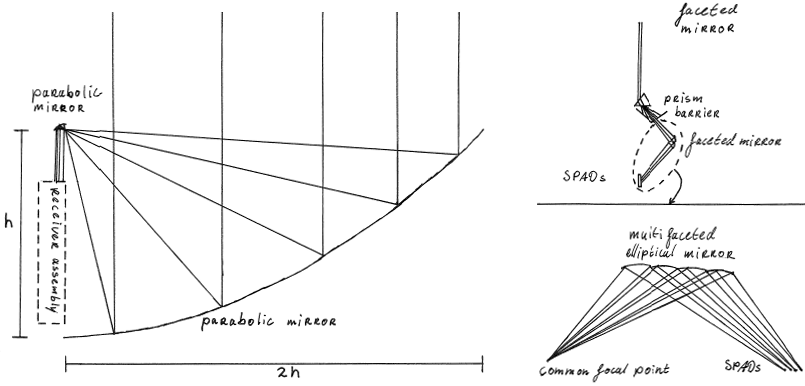
\includegraphics[scale = 0.5]{chapters/img/DiagramReceiverGeneral.png}
\caption{Receiver optics overview}
\label{fig:receiver_overview}
\end{figure} 

\subsection{Introduction}
\subsubsection{Design Concept}
The design concept for the optical receiving payload is demonstrated in figure \ref{fig:receiver_overview}, page \pageref{fig:receiver_overview}. Before going into this drawing, one first has to realize that a parabolic mirror takes parallel lightbeams and focuses them on a single focal point, or vice versa. Good examples of parabolic mirrors are solar collectors and satellite dishes.

Now in the left of figure \ref{fig:receiver_overview}, one can see the incident photons coming from the top. They are collected by the first parabolic reflector, which is the size of the receiver aperture, and sent through the focal point into the second parabolic mirror, top left. The second parabolic mirror has about the same focal point as the first parabolic mirror, and it is adjusted so that the light incident on it is transformed into a very tight parallel beam. The width of this focused beam is one millimeter.

The tight beam passes into the receiver assembly, the box shown to the utmost left of the figure. This assembly is enlarged in the top right of the drawing. The light beam passes through the prism which diffracts and filters out the light that is not in the required bandwidth. The exact working of this filter will be explained in section \ref{prism} After passing through the hole in the barrier, the filtered light is ready to be received by the \acp{SPAD}.

This part is enlarged on the right bottom of the drawing. The challenge here is to take the single coherent beam of light and spread it correctly over 32 by 32 widely spaced micron-scale detectors. This problem is solved by spreading the light out by a lens (not shown in the drawing), and then letting it fall on a 32 by 32 faceted array of elliptical mirrors.

Elliptical mirrors have a very interesting property: they take light coming from one focal point and focus it on the other focal point. The faceted mirror consists of elliptical mirrors, each of them having a commong focal point, which is the imaginary focal point behind the concave lens. Now whereas all 1024 elliptic facets have the first focal point in common, their second focal point is aligned, for every one of them, with their own detector in the 32 by 32 detector array. This allows subsampling of the beam onto the \ac{SPAD} array.

As the receiver orbit will drop over time, the focusing of the optical receiving payload has to be changed periodically. For this end, a linear actuator is put behind the secondary mirror, which refocuses it to keep the beam parallel when necessary. The design for this linear actuator is the same as for the laser focusing, so the reader is referred to section \ref{focus}, page \pageref{focus} for more detail.

\subsubsection{Performance Considerations}
The optical receiving payload has to perform well enough for the mission to deliver what its customers expect from it. This section explores what the impact of the payload design is on performance.

Firstly, the worst case resolution for the detector array is 97 picoseconds. This corresponds to a height of less than 3 centimeters, which is very good. This means that, once noise is filtered out, topology can be determined very accurately.

Secondly, the fact that the system uses an array of a 1024 detectors brings some interesting benefits to the platform. Not only does it allow the pointing requirements to be less stringent, but it also allows one to look within the footprint. The pointing accuracy is one tenth of a degree, which is about 870 meters on the Earth radius. There are 32 by 32 detectors, which means that a single detector will look at a 27 by 27 meter area. The laser dictating a footprint of 72 meters, this means that in total 9 to 16 detectors will be looking at the footprint at any time. This seems little - at most 16 out of 1024 detectors looking at the footprint. But as the number of photons per satellite per pulse is around, this is justificable.

The footprint subsampling allows the payload to not alone determine the terrain slope along the groundtrack of the emitter, but also cross-track. This allows determination of the (averaged) surface normal. In turn, this terrain surface normal allows much more precise determination of the \ac{BRDF}.

Another help here is the oversampling done by the constellation. At a forward speed of 8 km/s, and a sampling rate of 5 kHz, one finds that a footprint of 72 meters is imaged 45 times. This allows sophisticated averaging techniques, leading to precise terrain topology reconstruction, surface reflection characteristics determination, and \ac{BRDF} computation.

\subsection{\ac{SPAD}}
\label{SPAD}
A \acl{SPAD} identifies a class of solid-state photon detectors based on a reverse biased \textit{p-n junction} in which a photon-generated carrier can trigger an avalanche current due to the impact ionization mechanism. This device is able to detect low intensity signals (down to a single photon) and to signal the arrival times of the photons with a jitter of a few tens of picoseconds. However, these devices are typically based on complex circuits, whose area occupation and power consumption makes their integration impossible at the pixel level. In this case, 32 \acp{TDC} have been implemented on chip serving an array of 128x128 SPAD based pixels, while reports show an example of an in-pixel implementation, in a linear array, of a \ac{TAC} (\cite{SPAD3}). Figure \ref{fig:spad_overview} on page \pageref{fig:spad_overview} shows what the \acs{SPAD} chip looks like.

\begin{figure}[ht!]
\centering
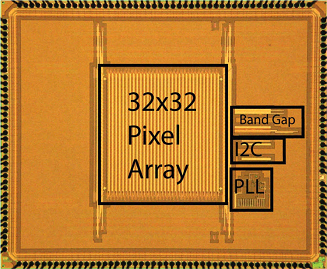
\includegraphics[scale = 0.8]{chapters/img/32by32array.png}
\caption{\acs{SPAD} chip photon-micrograph}
\label{fig:spad_overview}
\end{figure} 

\subsubsection{Avalanche Diodes}
\label{diodes}	
\aclp{SPAD} consist of avalanche diode. An avalanche diode is a \textit{p-n junction}, which has a voltage applied so that a single photon striking the depletion layer is amplified to a sustained avalanche. The start of the avalanche marks the arrival time of the photon. The avalanche is sustained until the diode is quenched.

Quenching is done by reversing the voltage to normal bias, which effectively wipes the diode, so that there is no avalanche any more and the device is light sensitive again. Quenching in our array is active. This reduces the dead time to values well below the 100 picosecond mark.

An avalanche may also be caused thermally. This is called \textit{dark noise}. As it increases with temperature, this means that for the receiver the lowest operable temperature is favoured. In space, this is not hard to achieve for such a low power chip. Additional dark noise is generated by stored charges, caused by quenching and avalanches.

A lot more can be said about avalanche diodes, but this report is not the place to do so. For more information, the reader can refer to the excellent work by those who built the chip we use: \cite{SPAD}, \cite{SPAD2} and \cite{SPAD3}.

\subsubsection{Space Qualification}
\label{SQ}
As the photon detection device will be operated in space, a big advantage of the 32$\times$32 pixel array \ac{SPAD} is that it was tested according to the \acsp{ESA} space qualification test. According to professor Charbon (\ac{SPAD} developer), the \ac{SPAD} chip itself survived during the test but not the motherboard connected to it, which means that a separate space application motherboard for the \ac{SPAD} chip needs to be designed.

\subsection{Prism Design}
\label{prism}
Before the prism is taken into consideration, the optical filter is also considered as an option, which is more simple than a prism and barrier system. The optical filter bandwidth accuracies are in terms of several tenths of nanometers, with a minimum of 10 nm (\cite{optical_filter}), which is not acceptable since the objective is to filter out all noise except for a 1 nm wavelength band around 473 nm both ways. Meanwhile, the transmission is another problem for normal optical filters, which have much lower values (of around 50\%) for smaller bandwidth accuracies (10 nm to 20 nm) and higher values (of around 90\%) for larger bandwidth accuracy (more than 30 nm), but prism can have transmissions as high as 97\% for the specified glass material.

Figure \ref{fig:prism} on page \pageref{fig:prism} gives an overview of the receiver optics after the second parabolic mirror. the prism is used to filter out all the noise light except those between 472 nm and 474 nm. The prism system needs to be accurate enough to perform the filtering within limited distance. The design contains the type of prism glass material, the incident angle $\alpha$, the prism apex angle $A$ and the distance between prism and barriers. They will be treated one by one.

\begin{figure}[ht!]
\centering
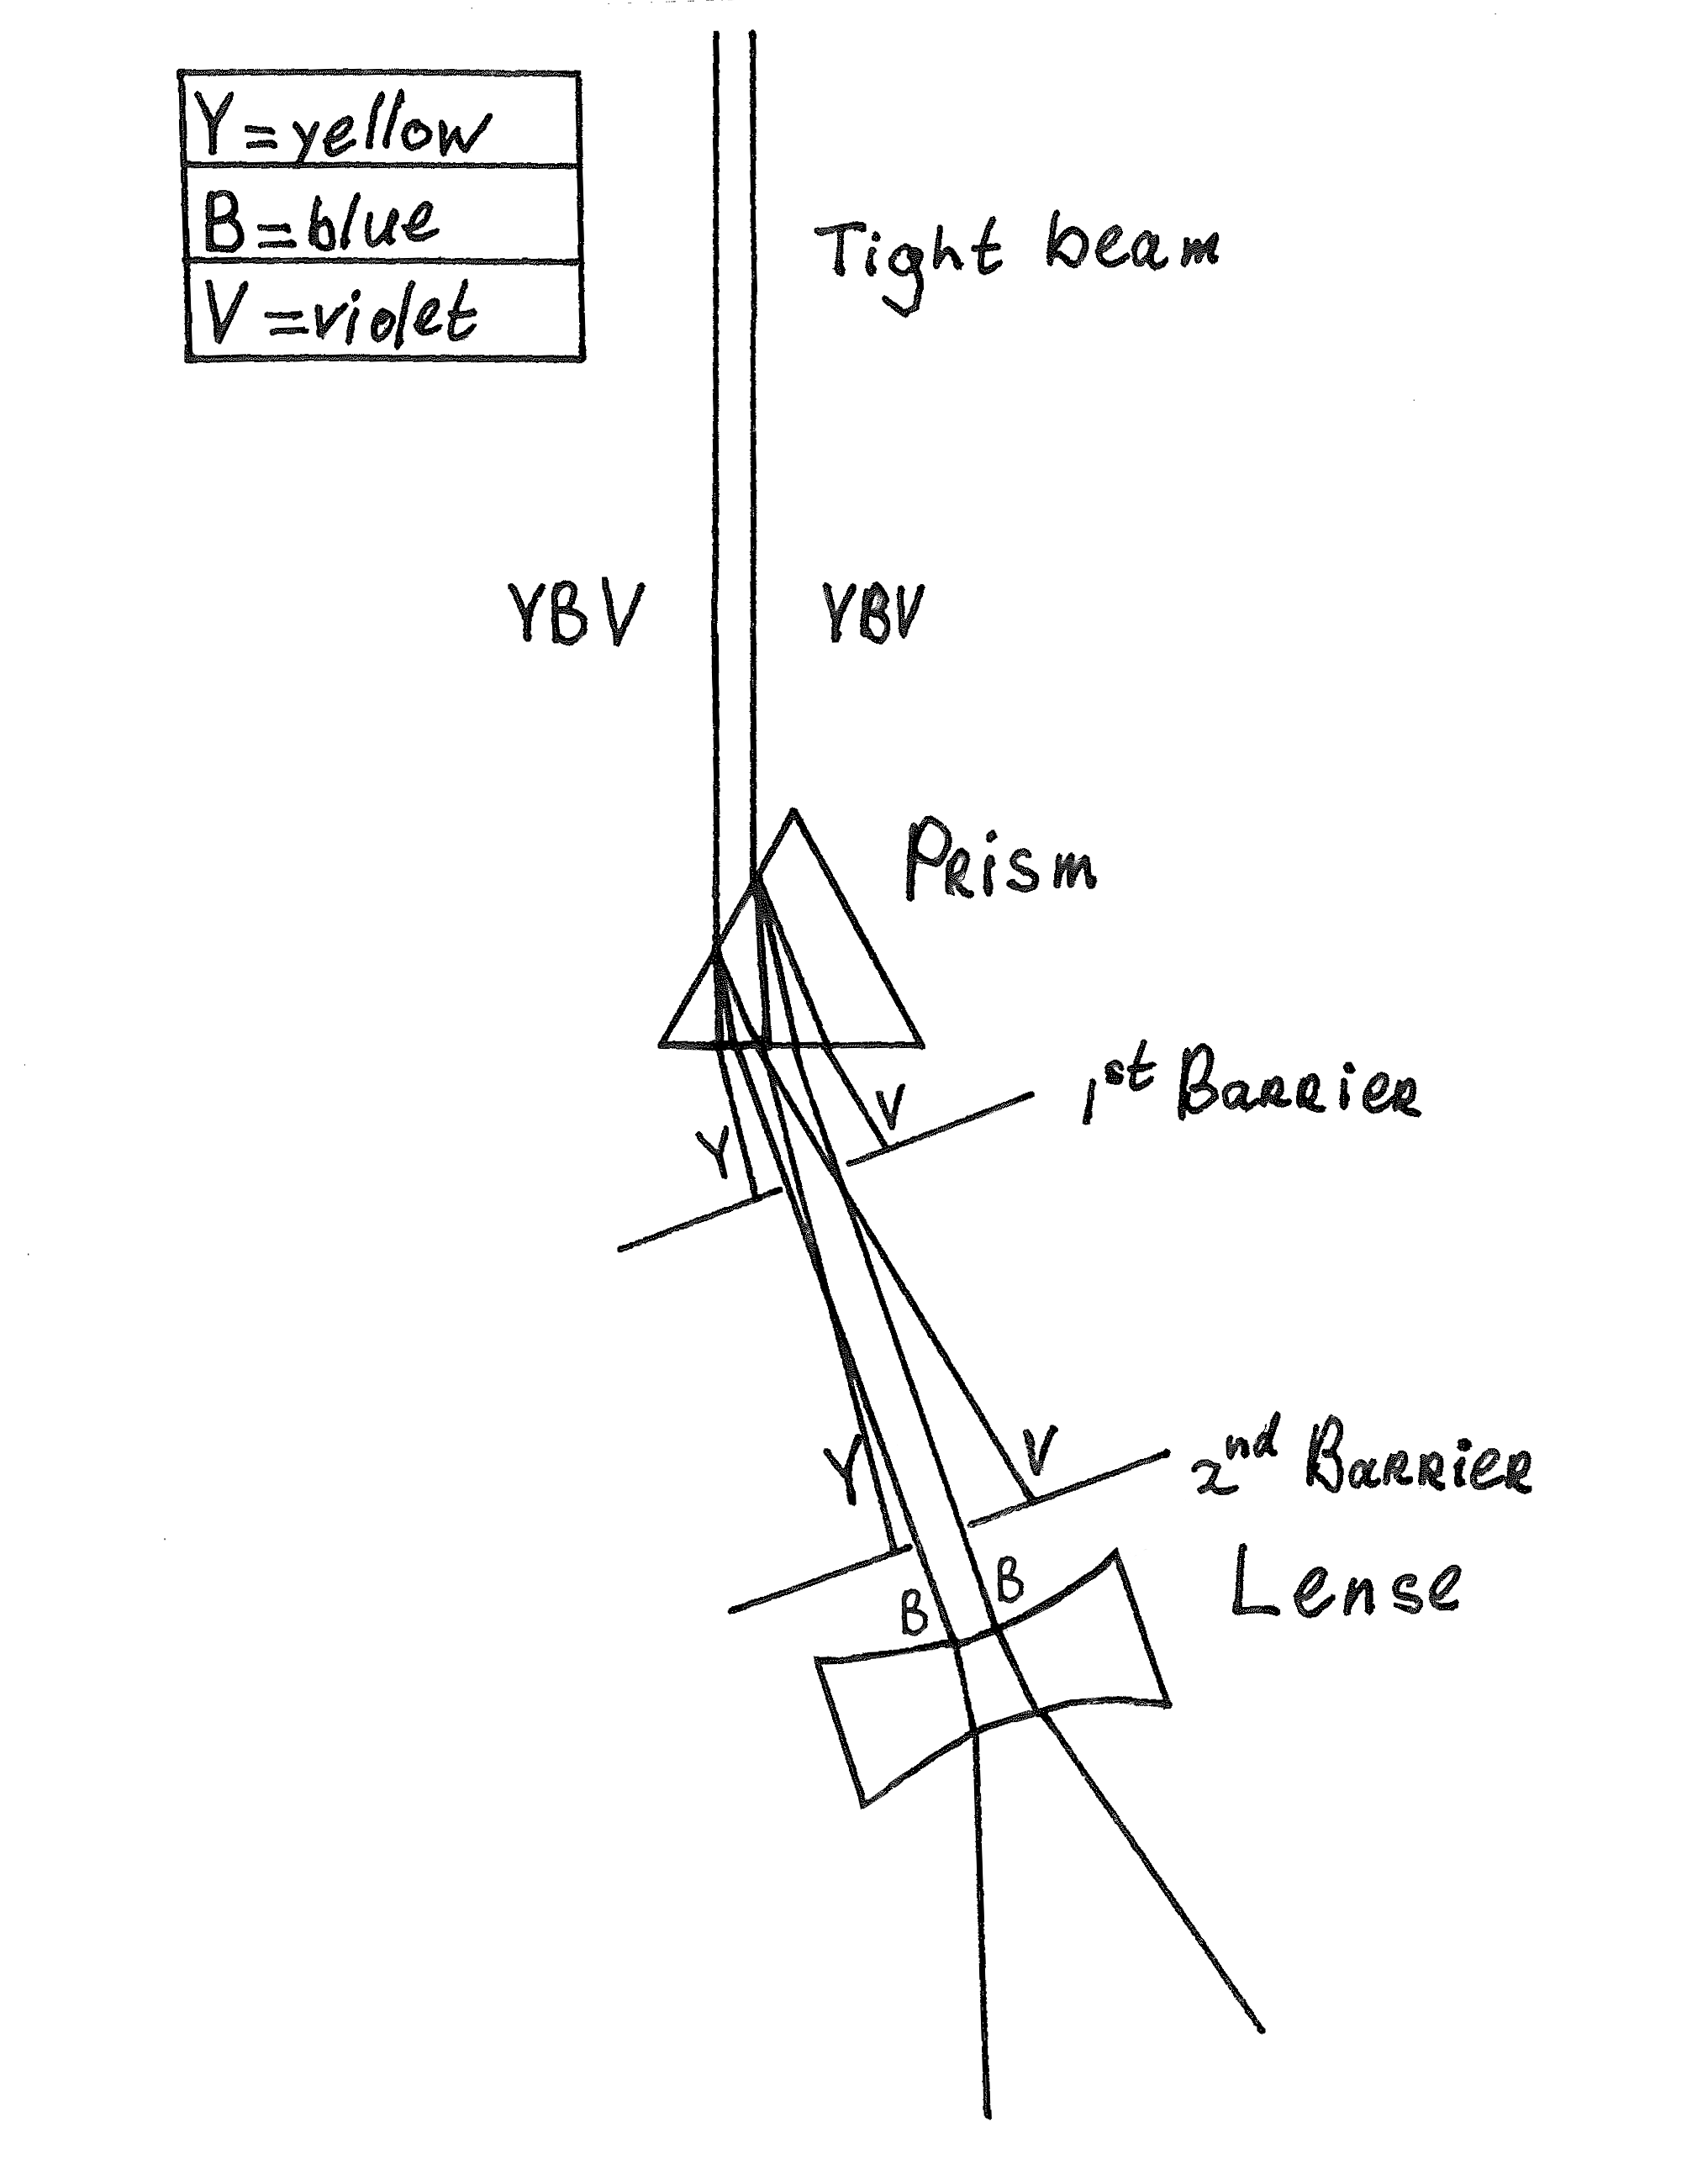
\includegraphics[scale = 0.6]{chapters/img/Prism.png}
\caption{Receiver prism filter overview}
\label{fig:prism}
\end{figure} 


\begin{figure}[ht!]
\centering
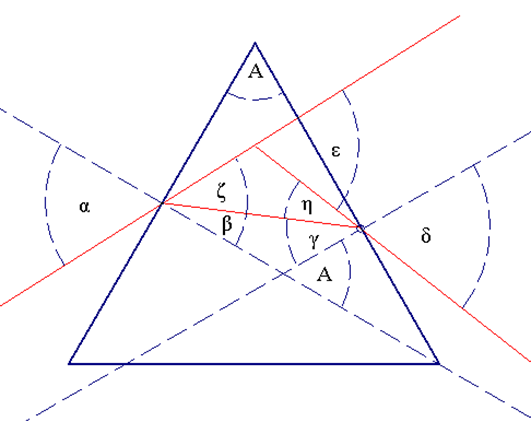
\includegraphics[scale = 0.6]{chapters/img/Prism2D.png}
\caption{Prism angles defined in 2D}
\label{fig:prism2D}
\end{figure} 
In figure \ref{fig:prism2D} on page \pageref{fig:prism2D}, the deviation angle $\epsilon$ can be calculated using the formula \cite{prism_angle_calculation}:
\begin{equation}
\label{epsilon}
\epsilon = \alpha - A + sin^{-1}(sin(A)\sqrt{n^2 - (sin(\alpha))^2} - cos(A)sin(\alpha))
\end {equation}
The key requirement to design the prism is to maximize the $\frac{d\epsilon}{d\lambda}$, because for a wavelength of 473 nm larger $\frac{d\epsilon}{d\lambda}$ leads to a smaller distance between prism and barriers. Equation \ref{epsilon} indicates that the deviation angle($\epsilon$) is a function of $A$, $\alpha$ and $n$. From Sellmeier's formula (see \cite{prism_book}), the index of refraction $n$ can be calculated to be:
\begin{equation}
\label{index_refraction}
n^2 - 1 = \frac{a_{1}\lambda^2}{\lambda^2-b_{1}} + \frac{a_{2}\lambda^2}{\lambda^2-b_{2}} + \frac{a_{3}\lambda^2}{\lambda^2-b_{3}}
\end {equation}
In the equation \ref{index_refraction}, $a_{1}, a_{2}, a_{3}$ and $b_{1}, b_{2}, b_{3}$ are the dispersion coefficients, which have different values for different glasses. In this case, the 17 most common prism glasses from the Schott company (see \cite{prism_material} and \cite{prism_book}) are analyzed. Since it is difficult to calculate $\frac{d\epsilon}{d\lambda}$ analytically, $\Delta\epsilon$ is calculated for the wavelengths of 472 nm, 473 nm and 474 nm can be obtained by inserting arbitrary A and $\alpha$, which is actually the $\frac{d\epsilon}{d\lambda}$ because the wavelength difference is only 1 nm of each. During the calculation, no matter what values are given for $A$ and $\alpha$, the SF11 glass always has the maximum value of $\Delta\epsilon$ which means it is the optimal choice of glass. Meanwhile, SF11 glass also has an internal transmittance of 97\% for wavelengths around 473 nm, which is acceptable.

The next step is to determine the prism apex angle $A$ and the incident angle $\alpha$. The prism apex angle is defined as $60^\circ$ because this gives the best average value for $\Delta\epsilon$. Meanwhile, this kind of equilateral prisms are also often used as dispersing prisms for wavelength separation applications(see figure \ref{fig:prism_equilateral} on page \pageref{fig:prism_equilateral}). 

\begin{figure}[ht!]
\centering
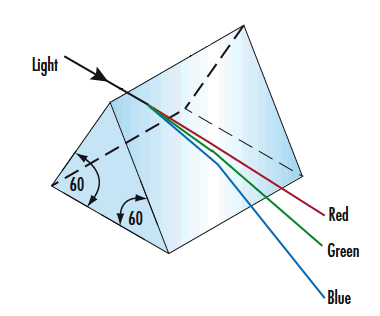
\includegraphics[scale = 0.8]{chapters/img/prism_equilateral.png}
\caption{Equilateral prism for wavelength separating applications. \emph{(Source: \cite{prism_material})}}
\label{fig:prism_equilateral}
\end{figure}

To select the correct incident angle, figure \ref{fig:prism_alpha} on page \pageref{fig:prism_alpha} is used. In the figure, the blue line is the asymptote about $\alpha = 54^\circ$. To avoid the asymptote, $\alpha = 55^\circ$ is selected as the incident angle, which leads to $\epsilon = 76^\circ$ and $\Delta\epsilon = 2.1432\ mrad$. Figure \ref{tab:SF11} on page \pageref{tab:SF11} is a part of the calculation in the excel sheet. There are two $\Delta\epsilon$s in the calculation; $\Delta\epsilon1 = \epsilon(472\ nm) - \epsilon(473\ nm)$ whereas $\Delta\epsilon2 = \epsilon(473\ nm) - \epsilon(474\ nm)$. The driving $\Delta\epsilon$ is the smaller one, since it is the minimum requirement. Taking $\Delta\epsilon = 2.1432\ mrad$ into further calculation, in order to separate the wavelength around 473 nm, at 472 nm and 474 nm, a barrier radius (or beam width) of 1 mm leads to a distance of 466.7 mm between prism and barrier. To shorten the distance, more concentrated beams are needed from the second parabolic mirror, or several flat mirrors can also be used to redirect the beam in a limited area. The figure \ref{fig:prism_final} on page \pageref{fig:prism_final} shows the final design of all angles.

\begin{figure}[ht!]
\centering
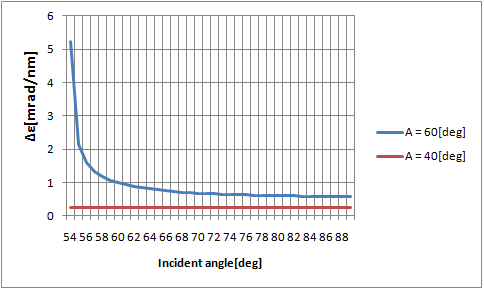
\includegraphics[scale = 1.2]{chapters/img/prism_alpha.png}
\caption{Plot of $\Delta\epsilon$ due to different incident angles}
\label{fig:prism_alpha}
\end{figure}

\begin{table}[ht!]
\centering
\begin{tabular}{ccc|ccc}
  a1 & a2 & a3 & b1 & b2 & b3 \\\hline
  1.74 & 0.31 & 1.17 & 0.0136 & 0.0616 & 0.0122 \\\\
  n(472 nm) & n(473 nm) & n(474 nm) & $\epsilon$(472 nm) & $\epsilon$(473 nm) & $\epsilon$(474 nm) \\\hline 
  1.81094 & 1.81061 & 1.81028 & 1.33596 & 1.33377 & 1.33162 \\\\
   \multicolumn{3}{c|}{$\Delta\epsilon$1 [mrad]} & \multicolumn{3}{c}{$\Delta\epsilon$2 [mrad]}\\\hline
  \multicolumn{3}{c|}{2.19189} & \multicolumn{3}{c}{\textbf{2.14316}} 
 \end{tabular}
\caption{Glass 'SF11' calculation parameters}
\label{tab:SF11}
\end{table}

\begin{figure}[ht!]
\centering
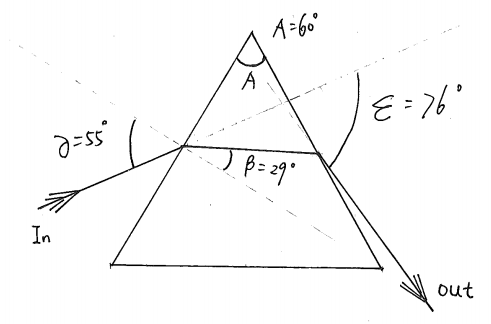
\includegraphics[scale = 0.8]{chapters/img/prism_final.png}
\caption{Overview of all angles}
\label{fig:prism_final}
\end{figure}

\subsection{Summary}
\label{sum}
The table \ref{tab:receiverbudget} on page \pageref{tab:receiverbudget} is the budget breakdown including mass and power consumption. To repeat, the large parabolic mirror is used to collect the reflected photons and the small parabolic mirror is used to create parallel tight beam before the prism. Flat mirrors are used after the prism to focus the light on faceted mirror. A separate cost estimation can be found in the section \ref{cost} on page \pageref{cost}.

\begin{table}[ht!]
\centering
\begin{tabular}{l | c | c | c | c }
\hline
Components                & Mass  & Quantity & Total mass & Power\\ 
                          &  [g]  &          &     [g]    &  [W] \\\hline\hline
Parabolic mirror (large)  &  95   &     1    &      95    &   0   \\
Parabolic mirror (small)  &  10   &     1    &     10     &   0   \\
Linear actuator		  &  5    &     1    &     5      &   0   \\
Faceted mirror            &  30   &     1    &     30     &   0   \\ 
Flat mirror               &  10   &     5    &     50     &   0   \\
\acs{SPAD}                &  10   &     1    &     10     &   0.1 \\
Prism                     &  10   &     1    &     10     &   0   \\ 
Concave lens              &  10   &     1    &     10     &   0   \\ \hline
Total                     &       &          &     220    &   0.1 \\\hline
\end{tabular}
\caption{Buget breakdown for receiver payload}
\label{tab:receiverbudget}
\end{table}


\subsection{Payload Cost Estimation}
\label{cost}
The table \ref{tab:cost_payload} on \pageref{tab:cost_payload} is the cost breakdown of the whole emitter and receiver payload system. The table is divided into 3 main parts.

The first part is the cost distribution of human resources. To design the payload prototype, different specific engineering skills are required with a salary of 122,380 \$ per manyear \cite{engineering_salary}. The 'Assessment manager' gains twice this salary, whereas the 'General manager' who is in charge of the whole project desires triple the salary of the normal engineers.

The second part is mainly about the manufacturing and production and the separate space qualification test that is required.

The third part first calculates the theoretical first unit cost of the receiver and the \acs{laser}, and then the obtained total cost of two types of combinations(5 receivers and 3 \acsp{laser} or 9 receivers and 3 \acsp{laser}) due to the learning curve effect \cite{Space2B}. It is obviously that the main cost of the payload is spent on the engineering design which is reasonable. For example, the final cost of 5 receivers and 3 \acsp{laser} would be $8.55 M\$ = a + b + c = 5.13996 + 2.92 + 0.49$; 9 receivers and 3 \acsp{laser} would lead to $8.66 M\$ = a + b + d = 5.13996 + 2.92 + 0.6$. Finally, the cost is scaled to American dollars in fiscal year 2000.

\begin{table}[ht!]
\centering
\begin{tabular}{p{0.9in}|cccccccccc||c}
&\begin{sideways}Electrical Engineering\end{sideways} 
&\begin{sideways}System Engineering\end {sideways} 
&\begin{sideways}Quality Engineering\end{sideways} 
&\begin{sideways}Material Engineering\end{sideways} 
&\begin{sideways}Software Engineering\end{sideways} 
&\begin{sideways}Mechanical Engineering\end{sideways} 
&\begin{sideways}Optical Engineering\end{sideways} 
&\begin{sideways}Thermal Engineering\end{sideways}
&\begin{sideways}Assessment Manager\end{sideways}
&\begin{sideways}General Manager\end{sideways}
&\begin{sideways}\textbf{Subtotal [M\$]}\end{sideways}\\\hline
\acs{SPAD} &2 &1 &1 &1 &2 &1 &0 &0 &1 &1 &1.8357 \\
Optics &0 &1 &1 &2 &0 &1 &1 &0 &1 &0 &0.97904 \\
\acs{laser} &3 &1 &2 &2 &2 &2 &3 &1 &1 &1 &2.32522 \\ \hline \hline 
Cost [M\$] &0.61 &0.37 &0.49 &0.61 &0.49 &0.49 &0.49 &0.12 &0.73 &0.73 &5.13996 (a) \\\hline\hline\\

&\begin{sideways}Integration and Test\end{sideways} 
&\begin{sideways}Space Qualification Test\end{sideways} 
&\begin{sideways}Product Assurance\end{sideways} 
&\begin{sideways}Material Cost\end{sideways} 
&\begin{sideways}Facilities/Machine\end{sideways}
&\begin{sideways}-\end{sideways} 
&\begin{sideways}-\end{sideways} 
&\begin{sideways}-\end{sideways} 
&\begin{sideways}-\end{sideways} 
&\begin{sideways}-\end{sideways}
&\begin{sideways}-\end{sideways}\\\hline
Receiver [M\$] &0.24 &0.3 &0.15 &0.01 &0.5 & & & & & &1.2 \\
\acs{laser} [M\$] &0.72 &0.3 &0.15 &0.05 &0.5 & & & & & &1.72 \\\hline\hline
Cost [M\$] &0.96 &0.6 &0.3 &0.06 &1 & & & & & &2.92 (b)\\\hline\hline\\

&\begin{sideways}Unit Cost\end{sideways} 
&\begin{sideways}5 Receiver\end{sideways} 
&\begin{sideways}9 Receiver\end{sideways} 
&\begin{sideways}-\end{sideways} 
&\begin{sideways}-\end{sideways}
&\begin{sideways}-\end{sideways} 
&\begin{sideways}-\end{sideways} 
&\begin{sideways}-\end{sideways} 
&\begin{sideways}-\end{sideways} 
&\begin{sideways}-\end{sideways}
&\begin{sideways}-\end{sideways}\\\hline
Receiver [M\$] &0.034 &0.15 &0.26 & & & & & & & & \\
\acs{laser} [M\$] &0.122 &0.34 &0.34 & & & & & & & & \\\hline\hline
Cost [M\$] &0.156 &0.49 (c) &0.6 (d) & & & & & & & &\\\hline\hline\\
\textbf{Total [M\$]} & &8.55 &8.66 & & & & & & & &\\\hline\\
\textbf{Total [FY00M\$]} & &6.98 &7.07 & & & & & & & &\\
\end{tabular}
\caption{Cost breakdown for emitter and receiver payload}
\label{tab:cost_payload}
\end{table}